%%%%%%%%%%%%%%%%%%%%%%%%%%%%%%%%%%%%%
%% Master Thesis - Computer Engineering
%% Copyright 2009 Ricardo Alexandre Fiorelli, Erick Poletto
%% This document is distributed by the terms of the license
%% included in the file LICENCE.
%%%%%%%%%%%%%%%%%%%%%%%%%%%%%%%%%%%%%

%%%%%%%%%%%%%%%%%%%%%%%%%%%%%%%%%%%%%
%% Third Chapter
%% Methodology
%%%%%%%%%%%%%%%%%%%%%%%%%%%%%%%%%%%%%

\chapter{Methodology} \label{chap3:methodology}

	This chapter will describe the steps taken to the end of constructing the components database and of validating the data contained in it.
These can be shortly described as follows:
    \begin{description}
        \item[Phase 0: Project definition -] As this work is part of a project aimed to create a methodology to implement a green ICT strategy, this first phase consisted of the definition of the logical components of this project and of how the current work would collaborate to it.
        \item[Phase 1: Analysis of Benchmarking Softwares -] A number of existing softwares were analyzed and those that have proven to be more adequate were selected. A list of the analyzed softwares can be found in Appendix~\ref{app:list_other_energy_management_tools}.
        \item[Phase 2: Catalog -] The tools were used to obtain information about computer components that were later used to create a component database.
        \item[Phase 3: Database design and construction -] The database schema was designed and data began to be inserted into the relations.
        \item[Phase 4: Analysis -] The validity of the stored data was tested with the help of direct measurements.
    \end{description}


\section{Overview} \label{sec3:overview}
    The main and broader objective of the research that is being conducted is to develop a methodology to implement a green ICT strategy. Namely, the methodology would provide a set of tools to guide the hardware acquisition process in an organization either in terms of workstations or of datacenter equipment. The present work will contribute to this research by providing a component database with information related to hardware components, which will be used as one of the inputs of the methodology. This work was conducted in order to determine how much energy a computer's components, for instance, CPU\footnote{Central Processing Unit}, Memory and Hard Drives spend and also how much they would affect the cost of acquisition of new computers as a whole. This is calculable with information such as component performance, power consumption and price. The analysis was carried out with the help of specialized softwares that will be described in the following sections and also with analytical measures made with an energy measurement device. In the end the benchmarking measures obtained from these softwares were compared with both the measures obtained from the device and with information provided by the component datasheets. With the benchmarking software, more than 1000 components were categorized in a database, whose schema can be found in Figure~\ref{fig:database_schema}. Firstly, the Sisoft Sandra's database~\ref{sec3:sandra} was used to collect the components and separate them by categories, along with their benchmark related data. Secondly, WebSPHINX~\ref{sec3:websphinx} was used to create a collection of components and their respective MPNs. In the end, an energy measurement device~\ref{sec3:energy_measurement_instrument} was used for the comparison and validation of the results given by the other benchmarks and acquisition of new data. 

    Finally, these data were all linked in a database for later comparison. 

\section{Research Design} \label{sec3:research_design} 
    The experimental method of research was used in this study. Figure~\ref{fig:experimental_method_approach} draws the steps of the method used. To define the experimental type of research, Bryman \cite{bryman89} states that ``the experimental design (\ldots) allows the causal hypothesis that underpins the question to be examined'', which means that this method is a systematic and scientific approach to research in which the researcher manipulates one or more variables, controlling and measuring any changes in other variables. The emphasis given is on the results and analysis of the benchmarks provided and theirs measures. It allows to verify the thesis in which this work is based on, by making use of empirical methods changing the benchmark used and the purpose of it.
    \begin{figure}[!htb]
        \centering
            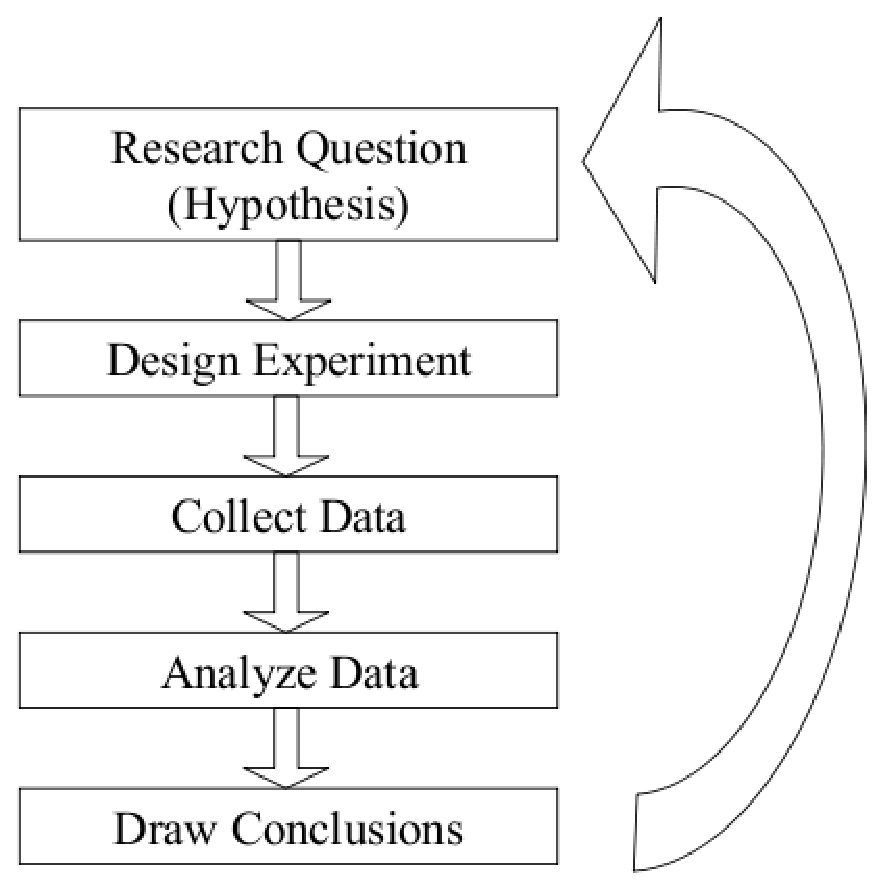
\includegraphics[scale=0.5]{graphics/experimental_method_approach}
            \caption{The Experimental Design Process}
            \label{fig:experimental_method_approach}
    \end{figure}

    % explicacao da figura

    %/********* Os proximos paragraphs foram criados para direcionar o pensamento e deve ser mantidos como comentario*******/
    %XXX

%    \item[Universe o Study] (whether a tribe, or a village, or an urban areas, or a particular group, etc.) - no nosso caso, os componentes do computador e o data center
    The present study was defined to identify the power consumption of the computer components in order to have a better tool to analyze the results of the measurements. The quantitative method (direct measurements and benchmarking), other than the qualitative method, was employed so as to identify the more energy efficient with the reason of building the most green data center and workstations. Among all components, the ones included in the measurements are: Chipset, Memory, Data Storage, Processor and the chassis (fan, power supply, etc).
%    \item[Subject of Study] (whether it focuses on the whole society, or any specific institution or a part of it).
    The choice of analyzing each component separately and also the whole computer power consumption was made in order to have a better control of the energy consumed and the ability to compare the different combination of components and, besides that, to obtain a representative amount of data for later analysis.
%    \item[Relationship Between certain variables] (Formulating a Research Design but it is not obligatory to start with a Research Design).

%    \item[Set of selected methods for obtain data] (whether participant observation, Interview, Questionnaire, or some other methods of data collection would be used).
    In order to obtain relevant data, three analysis' methods were used: empirical, benchmarking and research. For the empirical method, it was used an energy measurement device (section~\ref{sec3:energy_measurement_instrument}) that connected the electrical plug to the computer, and the measure was taken down in a spreadsheet%XXX
~\ref{tab:toolino_table}. While doing this, the benchmarking tool (section~\ref{sec3:sandra}) was performed in the host computer in order to acquire measures in a set of different situations. The last method, the research, the WebSPHINX, a web crawler was used in order to obtain information about the price and the MPN and with the objective of having a linked database provided by this code.
%    \item[Analytical Categories] (by which the empirical data is subjected to analysis and interpretation).
    In a later stage, all the data acquired by the measurement approaches were separated by categories and components. The database generated are explained in the section~\ref{sec3:data_processing_analysis}.
    
\section{Energy Management and Benchmarking Tools} \label{sec3:energy_management_tools}
    In order to obtain relevant information about the data required for making the comparison between the components, some energy management and benchmarking tools were used.
    
    The softwares that used were selected over the other available ones for their superior evaluation on the following criteria:
\begin{description}
	\item[Size of Database] The database of components used by the software, in order to get a good result, should be considerably large;
	\item[Characteristics of Benchmarks] The benchmarks provided by the software should provide information about the energy consumed for each component;
	\item[Number of Benchmarks] The software should have a good variety of benchmarks;
	\item[Quality of Benchmarks] Although the number of benchmarks should be sufficient in number, the quality, precision and relevancy were also important in the decision method;
	\item[Ease of Use] In the sense that the software should provide an ambient of work that is intuitive and comfortable;
\end{description}
    
    The acquisition of data was made analyzing the results of these benchmarks, making use of their database and system measurement capabilities.

    \subsection{SiSoftware SANDRA} \label{sec3:sandra}

    SiSoftware Sandra\footnote{The \textbf{S}ystem \textbf{AN}alyser, \textbf{D}iagnostic and \textbf{R}eporting \textbf{A}ssistant} is an information and diagnostic utility. It provides most of the information one need to know about their hardware, software and other devices whether hardware or software. SANDRA was the main software utilized to benchmark the data in this thesis work. It contains a vast database of components associated with both benchmark results and manufacturer specifications.
    
    The software goes beyond the point of other Windows Utilities, by giving the user, the possibility of benchmarking and comparing at both high and low level the computer devices. Moreover, it is a tool for monitoring the performance on systems and even benchmarking many parts of the computer, this includes, CPU, memory, hard disks, CD/DVD ROM, network, PSU, etc. For that reason, it is considered one of the most complete benchmarking tools available. Besides the benchmarking, Sandra also provides access to information about the Hardware, including the Motherboard, processor, disks, printers, etc; and Software, such as, key softwares (web browsers, e-mail program, etc.), OS information, processes, memory usage and more.
    
    The detailed list of modules utilized by SiSoftware Sandra can be found in Appendix~\ref{app:sandra_modules}.
    
    Furthermore, the Sandra has a great functionality that is a catalog of pricing, which, in addition to the power consumption and other important characteristics, the best combination (which means the most green) of devices can be chosen to the server.
    
    \subsection{Energy Measurement Instrument} \label{sec3:energy_measurement_instrument}

        \begin{figure}[!htb]
            \centering
                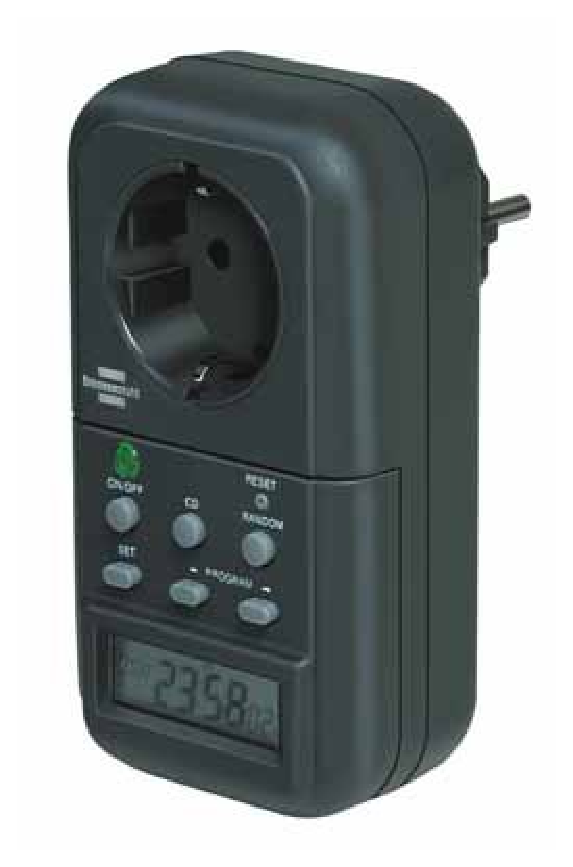
\includegraphics[scale=0.6]{graphics/energy_measurement_instrument}
                \caption{Energy Measurement Instrument}
                \label{fig:energy_measurement_instrument}
        \end{figure}
    The device, which can be seen on Figure~\ref{fig:energy_measurement_instrument}, was used for comparing and validating with the results of the benchmarks given by Sandra.

    After the result of the benchmark was obtained from the SiSoftware Sandra, this equipment that was connected to the computer read how much energy it was consumed and it was inserted in the database.
    
    %Quando Explicar sobre o database do toolino 
    \textbf{-colocar tabela do toolino e com o label ``tab:toolino\_table''}
    
    
        % TODO
    \subsection{WebSPHINX - A Personal, Customized Web Crawler} \label{sec3:websphinx}
        WebSPHINX\footnote{Website-Specific Processors for HTML Information Extraction} is a Java class library used for web crawling. It provides a way to browse and process web pages automatically.
        
        This piece of software was used to establish the pricing, linking it with the MPN\footnote{Manufacturer's Part Number}, and, afterwards, composing the database explained in \ref{sec4:analysis}. 
        % TODO
    
    \subsection{CPU-Z} \label{sec3:cpu-z}
        CPU-Z detects information about the CPU, RAM Memory, motherboard, chip-set and more. That program was used to complete the database with missing information about the components.
        % TODO

\section{Data Processing and Analysis} \label{sec3:data_processing_analysis}
    % TODO
    % explicar sobre a tabela geralzona que linka todos os componentes.
    % se nao colocar aqui, mudar para o capitulo 4.
